\mysection[Dandelion]{\centering Differenzierbare Funktionen}
Sei $D\subseteq\mathbb{R},f:D\rightarrow\mathbb{R},x_0\in D$ Häufungspunkt von $D$.

\DEF{Differenzen-Quotient}{Der Differenzen-Quotient $\frac{\Delta f}{\Delta x}=\frac{f(x)-f(x_0)}{x-x_0}$ ist die Steigung der Geraden durch $(x_0,f(x_0)),(x,f(x))$.}

\begin{figure}[H]
 \centering
 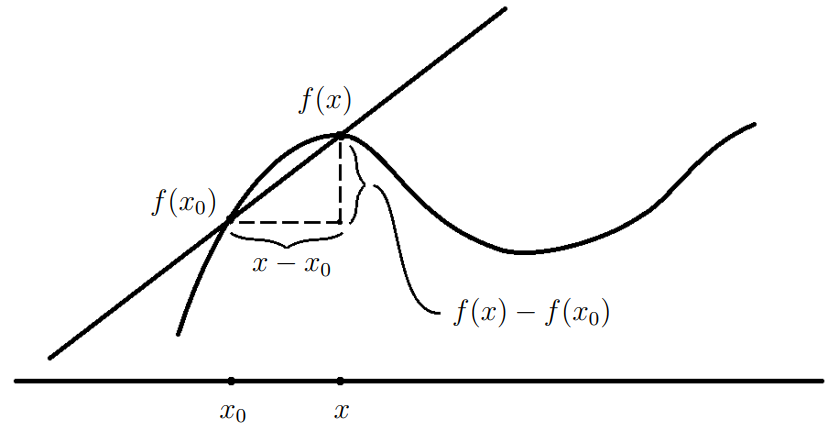
\includegraphics[width=\linewidth,keepaspectratio]{pictures/differenzen_quotient.png} 
\end{figure}

\DEF{Differenzierbar}{$f$ ist in $x_0$ differenzierbar, falls $\exists\ f'(x_0):=lim_{x\rightarrow x_0}\frac{f(x)-f(x_0)}{x-x_0}$.}

\NOTE{4.1.2}{Oftmals wird $f'(x_0)$ mit $x=x_0+h$ geschrieben: $f'(x_0)=lim_{h\rightarrow 0}\frac{f(x_0+h)-f(x_0)}{h}$.}

\SA{4.1.3}{Folgende Aussagen sind äquivalent:
\begin{enumerate}
    \item $f$ ist in $x_0$ differenzierbar.
    \item $\exists\ c\in\mathbb{R},\ r:D\rightarrow\mathbb{R}:$
    \begin{enumerate}
        \item[2.1] $f(x)=f(x_0)+c(x-x_0)+r(x)(x-x_0)$,
        \item[2.2] $r(x_0)=0 \land r$ stetig in $x_0$.
    \end{enumerate}
\end{enumerate}
Aus 2.1 folgt, dass $y=f(x_0)+f'(x_0)(x-x_0)$ die Gleichung der Tangente zum Graph von $f$ in $(x_0,f(x_0))$ ist. Wir können 2.1 noch Vereinfachen durch $\phi(x)=f'(x_0)+r(x)$.}

\SA{4.1.4}{$f$ in $x_0$ differenzierbar $\Leftrightarrow$ $\exists\ \phi:D\rightarrow\mathbb{R}$ die in $x_0$ stetig mit $f(x)=f(x_0)+\phi(x)(x-x_0)\ \forall x\in D$. Dann gilt $\phi(x_0)=f'(x_0)$.}

\COR{4.1.5}{$f$ in $x_0$ differenzierbar $\Rightarrow$ $f$ in $x_0$ stetig.}

\EXAMPLE{4.1.6}{
\begin{enumerate}
    \item $f=1:\mathbb{R}\rightarrow\mathbb{R},$ dann $f(x)-f(x_0)=1-1=0 \Rightarrow f'(x_0)=0\ \forall x_0\in\mathbb{R}$.
    \item $f:\mathbb{R}\rightarrow\mathbb{R},x\mapsto x,$ dann $f(x)-f(x_0)=x-x_0 \Rightarrow f'=1$.
    \item $f:\mathbb{R}\rightarrow\mathbb{R},x\mapsto x^2,$ dann $f(x)-f(x_0)=x^2-x_0^2=(x-x_0)(x+x_0)$. Somit für $x\not = x_0: \frac{f(x)-f(x_0)}{x-x_0}=x+x_0 \Rightarrow lim_{x\rightarrow x_0}\frac{f(x)-f(x_0)}{x-x_0}=lim_{x\rightarrow x_0}(x+x_0)=2x_0=f'(x_0)\ \forall x_0\in\mathbb{R}$.
    \item .
    \item .
\end{enumerate}}

\DEF{4.1.7}{$f:D\rightarrow\mathbb{R}$ ist in $D$ differenzierbar, falls $\forall$ Häufungspunkte $x_0\in D$, $f$ in $x_0$ differenzierbar.}

\EXAMPLE{4.1.8/10/13}{
\begin{enumerate}
    \item $(x^n)'=nx^{n-1}\ \forall n\geq 1,\ \forall x\in\mathbb{R}$.
    \item $exp'=exp$.
    \item $ln'(x)=\frac{1}{x}$.
    \item $sin'=cos$, $cos'=-sin$.
    \item $tan'(x)=\frac{1}{cos^2(x)}\ \forall x\not\in\frac{\pi}{2}+\pi\mathbb{Z}$.
    \item $cot'(x)=\frac{-1}{sin^2(x)}\ \forall x\not\in\pi\mathbb{Z}$.
    \item $arcsin'(x)=\frac{1}{\sqrt{1-x^2}}\ \forall x\in(-1,1)$.
    \item $arccos'(x)=\frac{-1}{\sqrt{1-x^2}}\ \forall x\in(-1,1)$.
    \item $arctan'(x)=\frac{1}{1+x^2}\ \forall x\in(-\infty,\infty)$.
    \item $arccot'(x)=\frac{-1}{1+x^2}\ \forall x\in(-\infty,\infty)$.
    \item $cosh'(x)=sinh(x)$, $sinh'(x)=cosh(x)$.
    \item $arcosh'(x)=\frac{1}{\sqrt{x^2-1}}\ \forall x\in(1,\infty)$.
    \item $arsinh'(x)=\frac{1}{\sqrt{x^2+1}}\ \forall x\in\mathbb{R}$.
    \item $artanh'(x)=\frac{1}{1-y^2}\ \forall y\in(-1,1).$
\end{enumerate}}

\SA{4.1.9}{Sei $D\subseteq\mathbb{R}, x_0\in D$ Häufungspunkt von $D$, $f,g:D\rightarrow\mathbb{R}$ in $x_0$ differenzierbar, $c\in\mathbb{R}$ konstant. Dann
\begin{enumerate}
    \item $c\cdot f,f+g$ in $x_0$ differenzierbar und 
    $(c\cdot f)'(x_0)=c\cdot f'(x_0)$, $(f+g)'(x_0)=f'(x_0)+g'(x_0)$.
    \item $f\cdot g$ in $x_0$ differenzierbar und $(f\cdot g)'(x_0)=f'(x_0)g(x_0)+f(x_0)g'(x_0)$.
    \item Falls $g(x_0)\not = 0$ ist $\frac{f}{g}$ in $x_0$ differenzierbar und $(\frac{f}{g})'(x_0)=\frac{f'(x_0)g(x_0)-f(x_0)g'(x_0)}{g(x_0)^2}$.
\end{enumerate}}


\SA{4.1.11 (Kettenregel)}{Seien $D,E\subseteq\mathbb{R}, x_0\in D$ ein Häufungspunkt. Sei $f:D\rightarrow E$ in $x_0$ differenzierbar s.d. $y_0:=f(x_0)$ ein Häufungspunkt von $E$. Sei $g:E\rightarrow\mathbb{R}$ eine in $y_0$ differenzierbare Funktion. Dann $g\circ f:D\rightarrow\mathbb{R}$ in $x_0$ differenzierbar und $(g\circ f)'(x_0)=g'(f(x_0))f'(x_0)$.}

\COR{4.1.12}{Sei $f:D\rightarrow E$ bijektiv, $x_0\in D$ Häufungspunkt. Angenommen $f$ in $x_0$ differenzierbar, $f'(x_0)\not = 0$, und $f^{-1}$ in $y_0=f(x_0)$ stetig. Dann $y_0$ Häufungspunkt von $E$, $f^{-1}$ in $y_0$ differenzierbar und $(f^{-1})'(y_0)=\frac{1}{f'(x_0)}$.}

\DEF{Lokale Maxima/Minima}{Sei $D\subseteq\mathbb{R},f:D\rightarrow\mathbb{R},x_0\in D$.
\begin{enumerate}
    \item $\exists\delta > 0: f(x)\leq f(x_0)\ \forall x\in (x-\delta,x+\delta)\cap D$ $\Rightarrow x_0$ ist lokales Maximum von $f$.
    \item $\exists\delta > 0: f(x)\geq f(x_0)\ \forall x\in (x-\delta,x+\delta)\cap D$ $\Rightarrow x_0$ ist lokales Minimum von $f$.
    \item $x_0$ lokales Maximum $\lor$ $x_0$ lokales Minumum $\Rightarrow x_0$ lokales Extremum.
\end{enumerate}}

\DEF{Example}{Sei $f:[a,b]\rightarrow\mathbb{R}$ wie im nachfolgenden Bild. Dann sind $a,x_1,x_3$ lokale Minima und $x_0,x_2,b$ lokale Maxima.}
\begin{figure}[H]
 \centering
 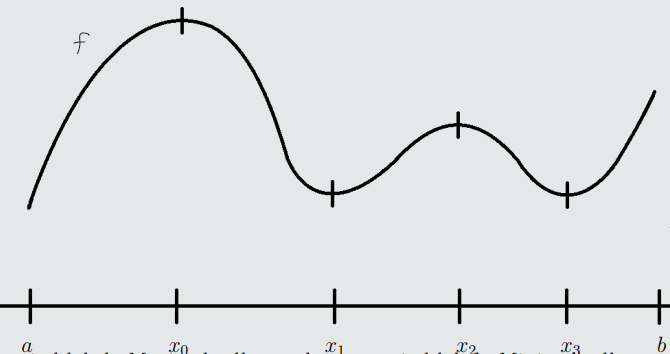
\includegraphics[width=\linewidth,keepaspectratio]{pictures/lokale_maxima_und_minima.png} 
\end{figure}

\DEF{Ableitungen von geraden und ungeraden Funktionen}{Sei $f:\mathbb{R}\rightarrow\mathbb{R}$. 

$f$ gerade $\Leftrightarrow f(-x)=f(x)\ \forall x\in\mathbb{R} \Rightarrow f'$ ungerade.

$f$ ungerade $\Leftrightarrow f(-x)=-f(x)\ \forall x\in\mathbb{R} \Rightarrow f'$ gerade.}


\SA{4.2.2}{Sei $D\subseteq\mathbb{R},x_0\in D$ Häufungspunkt von $D$, $f:D\rightarrow\mathbb{R}$ differenzierbar in $x_0$.
\begin{enumerate}
    \item $f'(x_0)>0\Rightarrow\ \exists\delta > 0:$\\
            $f(x)>f(x_0)\ \forall x\in (x_0,x_0+\delta)\cap D$,\\
            $f(x)<f(x_0)\ \forall x\in (x_0-\delta,x_0)\cap D$.
    \item $f'(x_0)<0\Rightarrow\ \exists\delta > 0:$\\
            $f(x)<f(x_0)\ \forall x\in (x_0,x_0+\delta)\cap D$,\\
            $f(x)>f(x_0)\ \forall x\in (x_0-\delta,x_0)\cap D$.
    \item $f$ besitzt lokales Extremum in $x_0$ $\land$ $x_0$ ist links- und rechtsseitiger Häufungspunkt von $D$ $\Rightarrow f'(x_0)=0$.
\end{enumerate}}

\SA{4.2.3 (Rolle 1690)}{Sei $a<b$, $f:[a,b]\rightarrow\mathbb{R}$ stetig und in $(a,b)$ differenzierbar. Wenn $f(a)=f(b) \Rightarrow\ \exists \xi\in(a,b)$ mit $f'(\xi)=0$.}

\SA{4.2.4 (Mittelwertsatz, Lagrange 1797)}{Sei $a<b$, $f:[a,b]\rightarrow\mathbb{R}$ stetig und in $(a,b)$ differenzierbar. Dann $\exists\ \xi\in(a,b)$ mit $f(b)-f(a)=f'(\xi)(b-a)\Leftrightarrow f'(\xi)=\frac{f(b)-f(a)}{b-a}$.}

\COR{4.2.5}{Sei $a<b,f,g:[a,b]\rightarrow\mathbb{R}$ stetig und in $(a,b)$ differenzierbar.
\begin{enumerate}
    \item $f'(\xi)=0\ \forall\xi\in(a,b) \Rightarrow f$ konstant.
    \item $f'(\xi)=g'(\xi)\ \forall\xi\in(a,b) \Rightarrow\exists c\in\mathbb{R}:f(x)=g(x)+c\ \forall x\in[a,b]$.
    \item $f'(\xi)\geq 0\ \forall\xi\in(a,b) \Rightarrow f$ auf $[a,b]$ monoton wachsend.
    \item $f'(\xi)>0\ \forall\xi\in(a,b) \Rightarrow f$ auf $[a,b]$ streng monoton wachsend.
    \item $f'(\xi)< 0\ \forall\xi\in(a,b) \Rightarrow f$ auf $[a,b]$ monoton fallend.
    \item $f'(\xi)\leq0\ \forall\xi\in(a,b) \Rightarrow f$ auf $[a,b]$ streng monoton fallend.
    \item $\exists M\geq 0:|f'(\xi)|\leq M\ \forall\xi\in(a,b) \Rightarrow \forall x_1,x_2\in[a,b]:|f(x_1)-f(x_2)|\leq M|x_1-x_2|$.
\end{enumerate}}

\SA{4.2.9 (Cauchy)}{Seien $a<b,f,g:[a,b]\rightarrow\mathbb{R}$ stetig und in $(a,b)$ differenzierbar. Dann $\exists \xi\in(a,b):g'(\xi)(f(b)-f(a))=f'(\xi)(g(b)-g(a))$. Falls $g'(x)\not = 0\ \forall x\in(a,b)$ $\Rightarrow g(a)\not = g(b) \land \frac{f(b)-f(a)}{g(b)-g(a)}=\frac{f'(\xi)}{g'(\xi)}$.}

\SA{4.2.10 (l'Hospital)}{Seien $a<b,f,g:(a,b)\rightarrow\mathbb{R}$ differenzierbar mit $g'(x)\not = 0\ \forall x\in(a,b)$. Falls $(lim_{x\rightarrow b^-}f(x)=lim_{x\rightarrow b^-}g(x)=0$ $\lor$ $(lim_{x\rightarrow b^-}f(x)= \pm\infty \land lim_{x\rightarrow b^-}g(x)=\pm\infty))$ $\land$ $\exists lim_{x\rightarrow b^-}\frac{f'(x)}{g'(x)}=:\lambda$ $\Rightarrow lim_{x\rightarrow b^-}\frac{f(x)}{g(x)}=lim_{x\rightarrow b^-}\frac{f'(x)}{g'(x)}$.

Der Satz gilt auch falls \begin{itemize}
    \item $b=\infty$,
    \item $a=-\infty$,
    \item $\lambda = \pm\infty$,
    \item $x\rightarrow a^+$.
\end{itemize}}

\DEF{Konvex}{Sei $I\subseteq\mathbb{R}$ ein Intervall mit mehr als einem Punkt und $f:I\rightarrow\mathbb{R}$.
\begin{enumerate}
    \item $x,y \in I, \forall x\leq y, \lambda\in[0,1]:f(\lambda x+(1-\lambda)y)\leq\lambda f(x)+(1-\lambda)f(y)$ $\Rightarrow f$ konvex auf $I$.
    \item $x,y \in I, \forall x<y, \lambda\in[0,1]:f(\lambda x+(1-\lambda)y)<\lambda f(x)+(1-\lambda)f(y)$ $\Rightarrow f$ streng konvex auf $I$.
\end{enumerate}}

\begin{figure}[H]
 \centering
 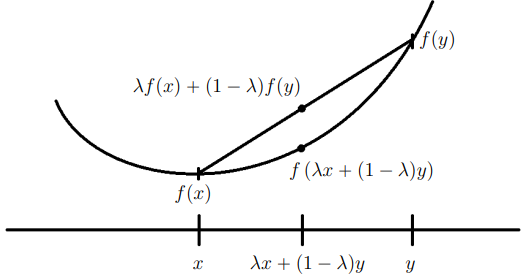
\includegraphics[width=\linewidth,keepaspectratio]{pictures/konvex.png} 
\end{figure}

\DEF{Konkav}{Sei $I\subseteq\mathbb{R}$ ein Intervall mit mehr als einem Punkt und $f:I\rightarrow\mathbb{R}$.

$-f$ (streng) konvex $\Rightarrow$ $f$ (streng) konkav.}

\NOTE{4.2.14}{Sei $f:I\rightarrow\mathbb{R}$ konvex. $\forall n\geq 1, \{x_1,...,x_n\}\subseteq I, \lambda_1,...,\lambda_n\in[0,1]$ mit $\sum_{i=1}^n\lambda_i=1$ gilt $f(\sum_{i=1}^n\lambda_ix_i)\leq\sum_{i=1}^n\lambda_if(x_i)$.}

\LEM{4.2.15}{Sei $f:I\rightarrow\mathbb{R}$ beliebig. Dann 
\begin{enumerate}
    \item $f$ konvex $\Leftrightarrow$ $\forall x_0<x<x_1\in I:$ $\frac{f(x)-f(x_0)}{x-x_0}\leq\frac{f(x_1)-f(x)}{x_1-x}$,
    \item $f$ streng konvex $\Leftrightarrow$ $\forall x_0<x<x_1\in I:$ $\frac{f(x)-f(x_0)}{x-x_0}<\frac{f(x_1)-f(x)}{x_1-x}$,
    \item $f$ konkav $\Leftrightarrow$ $\forall x_0<x<x_1\in I:$ $\frac{f(x)-f(x_0)}{x-x_0}\geq\frac{f(x_1)-f(x)}{x_1-x}$,
    \item $f$ streng konkav $\Leftrightarrow$ $\forall x_0<x<x_1\in I:$ $\frac{f(x)-f(x_0)}{x-x_0}>\frac{f(x_1)-f(x)}{x_1-x}$.
\end{enumerate}}

\LEM{}{Sei $f:I\rightarrow\mathbb{R}$ und $x_0<x<x_1\in I$. Dann folgt aus L4.2.15: 
\begin{enumerate}
    \item $f$ konvex $\Rightarrow$ $\frac{f(x)-f(x_0)}{x-x_0}\leq\frac{f(x_1)-f(x_0)}{x_1-x_0}\leq\frac{f(x_1)-f(x)}{x_1-x}$. 
    \item $f$ konkav $\Rightarrow$ $\frac{f(x)-f(x_0)}{x-x_0}\geq\frac{f(x_1)-f(x_0)}{x_1-x_0}\geq\frac{f(x_1)-f(x)}{x_1-x}$. 
\end{enumerate}
Strenge Konvexität (Konkavität) impliziert $<$ ($>$) statt $\leq$ ($\geq$) in obigen Ungleichungen.}

\SA{4.2.16}{Seien $a<b$. Sei $f:(a,b)\rightarrow\mathbb{R}$ in $(a,b)$ differenzierbar. Dann
\begin{enumerate}
    \item $f$ (streng) konvex $\Leftrightarrow$ $f'$ (streng) monoton steigend, 
    \item $f$ (streng) konkav $\Leftrightarrow$ $f'$ (streng) monoton fallend.
\end{enumerate}
Gilt auch für geschlossene Intervalle.}

\COR{4.2.17}{Seien $a<b$. Sei $f:(a,b)\rightarrow\mathbb{R}$ in $(a,b)$ zweimal differenzierbar. Dann
\begin{enumerate}
    \item $f''\geq 0$ (bzw. $f''>0$) auf $(a,b)$ $\Rightarrow$ $f$ (streng) konvex,
    \item $f''\leq 0$ (bzw. $f''<0$) auf $(a,b)$ $\Rightarrow$ $f$ (streng) konkav.
\end{enumerate}}


\mysubsection{Höhere Ableitungen}
Sei $D\subseteq\mathbb{R}$ s.d jedes $x_0\in D$ Häufungspunkt von $D$ ist. Sei $f:D\rightarrow\mathbb{R}$ differenzierbar in $D$ und $f^{(1)}=f'$ ihre Ableitung.

\DEF{Höhere Ableitungen}{
\begin{enumerate}
    \item Für $n\geq 2$ ist $f$ n-mal differenzierbar in $D$ falls $f^{(n-1)}$ in $D$ differenzierbar. Dann ist $f^{(n)}:=(f^{(n-1)})'$ die $n$-te Ableitung von $f$.
    \item $f$ $n$-mal differenzierbar $\land\ f^{(n)}$ in $D$ stetig $\Rightarrow f$ $n$-mal stetig differenzierbar in $D$.
    \item $f\ \forall n\geq 1$ $n$-mal differenzierbar $\Rightarrow$ $f$ ist in $D$ glatt (smooth).
\end{enumerate}}

\NOTE{4.3.2}{Für $n\geq 1:$ $f$ $n$-mal differenzierbar $\Rightarrow$ $f\ (n-1)$-mal stetig differenzierbar. Somit sind glatte Funktionen $n$-mal stetig differenzierbar $\forall n\geq 1$.}

\EXAMPLE{4.3.4/7}{
\begin{enumerate}
    \item $exp,sin,cos,sinh,cosh,tanh$ sind glatt auf ganz $\mathbb{R}$.
    \item $tan$ ist auf $\mathbb{R}\setminus\{\frac{\pi}{2}+k\pi:k\in\mathbb{Z}\}$ glatt.
    \item $cot$ ist auf $\mathbb{R}\setminus\{k\pi:k\in\mathbb{Z}\}$ glatt.
    \item $arcsin, arccos, arctan, arccot$ sind glatt.
    \item Polynome sind auf ganz $\mathbb{R}$ glatt.
    \item $ln:(0,\infty)\rightarrow\mathbb{R}$ ist glatt. Es gilt $ln^{(n)}(x)=(-1)^{n-1}(n-1)!x^{-n}\ \forall n\geq 1$.
    \item $sqrt:[0,\infty)\rightarrow[0,\infty)$ ist glatt auf $(0,\infty)$.
\end{enumerate}}

\SA{4.3.3}{Sei $n\geq 1$. Sei $f,g:D\rightarrow\mathbb{R}$ $n$-mal differenzierbar in $D$. Dann
\begin{enumerate}
    \item $f+g$ ist $n$-mal differenzierbar und $(f+g)^{(n)}=f^{(n)}+g^{(n)}$.
    \item $f\cdot g$ ist $n$-mal differenzierbar und $(f\cdot g)^{(n)}=\sum_{k=0}^n{n\choose k}f^{(k)}g^{(n-k)}$.
\end{enumerate}}

\SA{4.3.5}{Sei $n\geq 1$. Sei $f,g:D\rightarrow\mathbb{R}$ $n$-mal differenzierbar in $D$. Sei $g(x)\not = 0$ $\forall x\in D$. Dann $\frac{f}{g}$ $n$-mal differenzierbar in $D$.}

\SA{4.3.6}{Seien $E,D\subseteq\mathbb{R}$ Teilmengen für die jeder Punkt Häufungspunkt ist. Seien $f:D\rightarrow\mathbb{E}$ und $g:E\rightarrow\mathbb{R}$ $n$-mal differenzierbar. Dann ist $g\circ f$ $n$-mal differenzierbar, und $(g\circ f)^{(n)}(x)=\sum_{k=1}^nA_{n,k}(x)(g^{(k)}\circ f)(x)$ wobei $A_{n,k}$ ein Polynom in den Funktionen $f',f^{(2)},...,f^{(n+1-k)}$ ist. Beispiele:

\begin{itemize}
    \item $(g\circ f)'=(g'\circ f)f'$.
    \item $(g\circ f)^{(2)}=(g^{(2)}\circ f)(f')^2+(g'\circ f)f^{(2)}$.
    \item $(g\circ f)^{(3)}=(g^{(3)}\circ f)(f')^3+3(g^{(2)}\circ f)f'f^{(2)}+(g'\circ f)f^{(3)}$.
\end{itemize}}

\mysubsection{Potenzreihen, Taylor Approximation}
\SA{4.4.1}{Sei $I\subseteq\mathbb{R}$. Seien $f_n:I\rightarrow\mathbb{R}$, $n\in\mathbb{N}^*$, stetig differenzierbar. Angenommen
\begin{enumerate}
    \item $(f_n)_{n\geq 1}$ konvergiert gleichmässig in $I$ gegen $lim_{n\rightarrow\infty}f_n=:f$,
    \item $(f'_n)_{n\geq 1}$ konvergiert gleichmässig in $I$ gegen $lim_{n\rightarrow\infty}f'_n=:p$.
\end{enumerate}
Dann $f$ stetig differenzierbar und $f'=p$.}

\SA{4.4.2}{Sei $\sum_{k=0}^{\infty}c_kx^k$ eine Potenzreihe mit $\rho > 0$. Dann ist $f(x)=\sum_{k=0}^{\infty}c_k(x-x_0)^k$ auf $(x_0-\rho,x_0+\rho)$ differenzierbar und $f'(x)=\sum_{k=1}^{\infty}kc_k(x-x_0)^{k-1}\ \forall x\in(x_0-\rho,x_0+\rho)$.}

\COR{4.4.3}{Unter der Voraussetzung von Satz 4.4.1 ist $f$ auf $(x_0-\rho,x_0+\rho)$ glatt und $f^{(j)}(x)=\sum_{k=j}^{\infty}c_k\frac{k!}{(k-j)!}(x-x_0)^{k-j}$. Insbesondere ist $c_j=\frac{f^{(j)}(x_0)}{j!}$.}

\EXAMPLE{4.4.4}{Nicht jede glatte Funktion ist Summe einer Potenzreihe.}

\DEF{Taylorpolynom}{Sei $I\in\mathbb{R}$ ein Intervall mit mehr als einem Punkt. Sei $n\in\mathbb{N},f:I\rightarrow\mathbb{R}$ $n$-mal differenzierbar. Sei $x_0\in I$. Dann ist das Tylorpolynom der Ordnung $n$ von $f$ in $x_0:$ $T_nf(x;x_0):=\sum_{k=0}^n\frac{f^{(k)}(x_0)}{k!}(x-x_0)^k$. $p:=T_nf(x;x_0)$ ist eindeutig mit
\begin{enumerate}
    \item $Grad(p)\leq n$.
    \item $f(x_0)=p(x_0),\ f'(x_0)=p'(x_0),\ ...,\ f^{(n)}(x_0)=p^{(n)}(x_0)$.
\end{enumerate}}

\SA{4.4.5 (Approximation glatter Funktionen)}{Sei $f:[a,b]\rightarrow\mathbb{R}$ stetig und in $(a,b)$ $(n+1)$-mal differenzierbar. Sei $x_0\in[a,b]$. Dann $\forall x\in[a,b],x\not=x_0\ \exists\xi$ zwischen $x_0$ und $x$ mit $f(x)=T_nf(x;x_0)+\frac{f^{(n+1)}(\xi)}{(n+1)!}(x-x_0)^{n+1}$.}

\COR{4.4.6 (Taylor Approximation)}{Sei $f:[a,b]\rightarrow\mathbb{R}$ $n$-mal stetig differenzierbar und in $(a,b)$ $(n+1)$-mal differenzierbar. Sei $x_0\in[a,b]$. Dann $\forall x\in[a,b],x\not=x_0\ \exists\xi$ zwischen $x_0$ und $x$ s.d. $f(x)=T_nf(x;x_0)+\frac{f^{(n+1)}(\xi)}{(n+1)!}(x-x_0)^{n+1}$.}

\DEF{Restglied der Taylor Approximation}{$f(x)-T_nf(x;x_0)$ wird als Restglied bezeichnet. Die Formel $\frac{f^{(n+1)}(\xi)}{(n+1)!}(x-x_0)^{n+1}$ ist die Restglieddarstellung von Lagrange.}

\COR{4.4.7}{Sei $n\geq 0, a<x_0<b$ und $f:[a,b]\rightarrow\mathbb{R}$ in $(a,b)$ $(n+1)$-mal stetig differenzierbar. Angenommen $f'(x_0)=f^{(2)}(x_0)=...=f^{(n)}(x_0)=0$.
\begin{enumerate}
    \item $n$ gerade $\land$ $x_0$ lokales Extremum $\Rightarrow$ $f^{(n+1)}(x_0)=0$,
    \item $n$ ungerade $\land$ $f^{(n+1)}(x_0)>0$ $\Rightarrow$ $x_0$ strikte lokale Minimalstelle,
    \item $n$ ungerade $\land$ $f^{(n+1)}(x_0)<0$ $\Rightarrow$ $x_0$ strikte lokale Maximastelle.
\end{enumerate}}

\COR{4.4.8}{Sei $f:[a,b]\rightarrow\mathbb{R}$ stetig und in $(a,b)$ zweimal stetig differenzierbar. Sei $a<x_0<b$. Angenommen $f'(x_0)=0$.
\begin{enumerate}
    \item $f''(x_0)>0$ $\Rightarrow$ $x_0$ striktes lokales Minima,
    \item $f''(x_0)<0$ $\Rightarrow$ $x_0$ striktes lokales Maxima.
\end{enumerate}}
